\chapter*{Dodatak: Prikaz aktivnosti grupe}
		\addcontentsline{toc}{chapter}{Dodatak: Prikaz aktivnosti grupe}
		
		\section*{Dnevnik sastajanja}
		
		\textbf{\textit{Kontinuirano osvježavanje}}\\
		
		 \textit{U ovom dijelu potrebno je redovito osvježavati dnevnik sastajanja prema predlošku.}
		
		\begin{packed_enum}
        \item Sastanak: 
            \item[] \begin{packed_item}
                \item Datum: 23. listopada 2023.
                \item Prisustvovali: Tea, Ian, Nikola, Ivan, Niko, Lovro, Karlo
                \item Teme sastanka:
                    \begin{packed_item}
                        \item \textbf{Prethodno Čitanje i Ažuriranja Tima:}
                            \begin{packed_item}
                                \item Ian: Napisao flow, pomagao s SpringBootom, komunikacija s asistentom
                                \item Tea: Odradila Git i Crash Courseve
                                \item Ivan: Istraživanje Gita, učenje Spring Boota
                                \item Lovro: Pregled video materijala, početak React tečaja
                                \item Niko: Rad s Gitom i konzolom, istraživanje Notiona
                                \item Nikola: Pregled sadržaja, planiranje dodatnih projekata
                                \item Karlo: Postavljanje Notiona, slušanje Spring predavanja, diskusija o flowu
                            \end{packed_item}
                        \item \textbf{Dnevni Red:}
                            \begin{packed_item}
                                \item Provjere gut osjećaja članova tima
                                \item Predavanja CROZ - prisustvovali Nikola i Karlo
                                \item Diskusija o procesu terapije i mogućnosti sudjelovanja djelatnika
                            \end{packed_item}
                        \item \textbf{Zaključci:}
                            \begin{packed_item}
                                \item Pacijenti biraju između preddefiniranih procedura terapije
                                \item Specijalizacija djelatnika za različite vrste procedura
                                \item Uloge liječnika i administrativnih djelatnika
                                \item Proces verifikacije podataka liječnika i registracije pacijenata
                                \item Implementacija sučelja za administracijske funkcije
                            \end{packed_item}
                        \item \textbf{Trajanje:} 60 minuta
                    \end{packed_item}
            \end{packed_item}
            
\vspace{30pt}

        \item Konzultacije s Asistentom:
        \item[] \begin{packed_item}
            \item Datum: 25. listopada 2023.
            \item Prisustvovali: Tea, Ian, Nikola, Ivan, Niko, Lovro (Karlo nije prisustvovao)
            \item Teme konzultacija:
                \begin{packed_item}
                    \item \textbf{Razrada i Pitanja:} [Detalji o postavljenim pitanjima i razgovoru]
                \end{packed_item}
            \item Zaključci sastanka:
                \begin{packed_item}
                    \item Git repozitorij treba biti javan s dodatnim suradnicima
                    \item Vođenje dnevnika sastanaka na Gitu s osnovnim informacijama
                    \item Korištenje lažne (fejk) baze podataka za provjeru liječnika
                    \item Šifriranje lozinki u bazi podataka
                    \item "Brisanje" računa u bazi podataka putem statusa
                    \item Referenciranje prethodnih terapija pomoću vanjskog ključa
                    \item Status liječnika odnosi se na aktivnost (npr. u penziji)
                    \item Izmisliti opremu, uređaje i terapije s realnim brojem resursa
                    \item Ciljevi do kraja prvog ciklusa: Deployment stranice, ostvarenje logina, minimalni prikaz podataka iz baze
                \end{packed_item}
            \item \textbf{Trajanje:} 60 minuta
        \end{packed_item}
\vspace{30pt}
        
        \item Diskusija: Use-Cases
            \item[] \begin{packed_item}
                \item Datum: 28. listopada 2023.
                \item Prisustvovali: Ian, Karlo (Niko, Nikola, Ivan, Lovro, Tea nisu prisustvovali)
                \item Teme diskusije:
                    \begin{packed_item}
                        \item \textbf{Real-Time Kalendar za Odabir Termina:}
                            \begin{packed_item}
                                \item Pacijenti biraju termine s obzirom na dostupnost djelatnika i opreme
                            \end{packed_item}
                        \item \textbf{Oprema i Prostor:}
                            \begin{packed_item}
                                \item Oprema i prostor tretirani su kao jedinstveni resurs (npr. bazen, elektroterapija)
                            \end{packed_item}
                        \item \textbf{Pravila za Odabir i Izmjenu Termina:}
                            \begin{packed_item}
                                \item Mogućnost izmjene termina s minimalnim vremenskim ograničenjem
                                \item Minimalni razmak između terapija definiran varijablama procedure
                            \end{packed_item}
                        \item \textbf{Proces Odobravanja Terapije:}
                            \begin{packed_item}
                                \item Provjera zdravstvenog osiguranja i ispravnosti odabrane terapije
                            \end{packed_item}
                        \item \textbf{Dilema oko Verifikacije:}
                            \begin{packed_item}
                                \item Diskusija o potrebi i načinu provođenja verifikacije tijekom registracije i prijave
                            \end{packed_item}
                    \end{packed_item}
                \item Zaključci sastanka:
                    \begin{packed_item}
                        \item Detaljno definiranje procesa odabira i izmjene termina
                        \item Razrada mehanizma odobravanja terapije
                        \item Rasprava o verifikaciji identiteta i osiguranja u kontekstu registracije i prijave
                    \end{packed_item}
                \item \textbf{Trajanje:} 60 minuta
            \end{packed_item}
        
\vspace{30pt}


        \item Sastanak: 
            \item[] \begin{packed_item}
                \item Datum: 29. listopada 2023.
                \item Prisustvovali: Tea, Ian, Nikola, Ivan, Niko, Lovro, Karlo
                \item Teme sastanka:
                    \begin{packed_item}
                        \item \textbf{Provjeravanje i Ažuriranja Tima:}
                            \begin{packed_item}
                                \item Tea: Analiza i proučavanje Ianovog koda, istraživanje LaTeXa
                                \item Nikola: Analiza Ianovog koda
                                \item Niko: Prati Scrimbu za dodatno učenje
                                \item Ivan: Proučava Ianov kod, instalira LaTeX editor
                                \item Lovro: Napreduje s Scrimbu tečajem
                                \item Ian: Objašnjava SpringBoot timu, priprema backend, uvoz podataka u bazu, planira deployment
                                \item Karlo: Ažuriranje GitHuba i Notiona, razrada flowa i use caseova
                            \end{packed_item}
                        \item \textbf{Dnevni Red i Ključna Pitanja:}
                            \begin{packed_item}
                                \item Stanje s dokumentacijom
                                \item Verifikacijski procesi pri registraciji i prijavi
                                \item Mogućnosti i funkcionalnosti pacijentovog dashboarda
                                \item Postojanje i funkcije liječničkog accounta
                                \item Mogućnosti i ovlasti djelatnika
                            \end{packed_item}
                        \item \textbf{Zaključci:}
                            \begin{packed_item}
                                \item Registracija pacijenata uz MBO i OIB
                                \item Definicija resursa i termina u kontekstu terapije
                                \item Funkcije i preglednost rasporeda za djelatnike
                                \item Detalji vezani uz profile pacijenata i djelatnika
                                \item Specifičnosti liječničkog accounta i pacijentovih mogućnosti na dashboardu
                            \end{packed_item}
                        \item \textbf{Trajanje:} 1 sat i 45 minuta
                    \end{packed_item}
            \end{packed_item}

\vspace{30pt}

        \item Sastanak:
    \item[] \begin{packed_item}
        \item Datum: 5. studenog 2023.
        \item Prisustvovali: Tea, Ian, Ivan, Niko, Lovro, Karlo (Nikola odsutan zbog operacije)
        \item Teme sastanka i Ažuriranja Članova Tima:
            \begin{packed_item}
                \item Tea: Uredila use-caseove u LaTeXu, postavila ih na GitHub, istraživanje baza podataka s Ianom
                \item Niko: Nastavak s tečajem Scrimbe
                \item Ivan: Napisao prvih 15 use-caseova
                \item Lovro: Završio Scrimbu, proučavao dokumentaciju
                \item Ian: Prošao use-caseove s Nikolom, razvio backend za registraciju i login, priprema za deployment
                \item Karlo: Organizacija Git-a, pisanje u Notionu, pregled use-caseova
            \end{packed_item}
        \item Razmatrana Pitanja:
            \begin{packed_item}
                \item Analiza use-caseova, posebno registracija i prijava bolesnika
                \item Pitanje upotrebe OIB-a i MBO-a u registraciji
                \item Use-case za prijavu u sustav i rezervaciju termina rehabilitacije
            \end{packed_item}
        \item Detaljni Zaključci:
            \begin{packed_item}
                \item Terapija veže uz sebe resurse: kombinacija slobodnog termina, resursa i djelatnika
                \item Djelatnici imaju opciju pisanja bilješki nakon termina
                \item Pacijenti imaju mogućnost pregleda i uređivanja svojih termina, s uvjetom promjene termina više od 48 sati unaprijed
                \item Administrativna provjera osiguranja bolesnika prema MBO-u pri prijavi na rehabilitaciju
                \item Otkazivanje termina uključuje dvosmjernu komunikaciju među svim ulogama
                \item Definiranje minimalnog razmaka između sesija i maksimalnog trajanja terapije
                \item Djelatnici u kalendaru vide samo svoje termine, s mogućnošću pretrage po pacijentu
                \item Nema privilegiranog djelatnika; svi djelatnici su ravnopravni u sustavu
                \item Specifični ciljevi za sljedeći ciklus: login, registracija, osnovna komunikacija s bazom
                \item Preispitivanje i optimizacija određenih use-caseova
            \end{packed_item}
        \item \textbf{Trajanje:} 2 sata
        \item \textbf{Todo:} Specifični zadaci dodijeljeni članovima tima
    \end{packed_item}

\vspace{30pt}

\item Sastanak za UI/UX
    \item[] \begin{packed_item}
        \item Datum: 12. studenog 2023.
        \item Teme Sastanka: UX/UI Dizajn i Dijagrami
        \item Prisustvovali: Niko, Karlo (Ian, Nikola, Ivan, Lovro, Tea nisu prisustvovali)
        \item Teme sastanka i Diskusije:
            \begin{packed_item}
                \item \textbf{Razvoj Korisničkog Sučelja:}
                    \begin{packed_item}
                        \item Razvijen UI za ključne stranice aplikacije, fokus na intuitivnosti i pristupačnosti
                        \item Detaljna diskusija o dizajnu i korisničkom iskustvu, uzimajući u obzir ciljanu publiku
                    \end{packed_item}
                \item \textbf{Dijagrami i Use-Caseovi:}
                    \begin{packed_item}
                        \item Diskutirani dijagrami s naglaskom na poboljšanje razumijevanja procesa unutar aplikacije
                        \item Niko zabilježio promjene i ažuriranja potrebna za use-caseove i dijagrame
                    \end{packed_item}
            \end{packed_item}
        \item Zaključci sastanka:
            \begin{packed_item}
                \item Uspješno razvijeno korisničko sučelje za početne stranice, usklađenost s općim ciljevima projekta
                \item Razrađeni dijagrami i vizualizacije procesa unutar aplikacije, povećanje transparentnosti i razumijevanja
                \item Ažuriranje i optimizacija use-caseova i dijagrama, osiguravajući njihovu usklađenost s trenutnim razvojem projekta
            \end{packed_item}
        \item \textbf{Trajanje:} 3 sata
        \item \textbf{Nastavak rada:} Fokus na daljnji razvoj UI/UX-a i finalizaciju dijagrama
    \end{packed_item}

\vspace{30pt}

\item Sastanak:
    \item[] \begin{packed_item}
        \item Datum: 13. studenog 2023.
        \item Prisustvovali: Tea, Nikola, Ivan, Niko, Lovro, Karlo (Ian nije prisustvovao zbog bolesti)
        \item Teme sastanka i Ažuriranja Članova Tima:
            \begin{packed_item}
                \item Tea: Uključivanje baze podataka u dokumentaciju, opis arhitekture, pisanje natuknica o projektu, priprema poglavlja 4.1 s opisom tablica
                \item Nikola: Pregled dijagrama i osiguravanje njihove točnosti
                \item Niko: Rad na use-case i sekvencijskim dijagramima, ispravci dokumentacije, suradnja s Karlom i Lovrom na Figmi, završetak Scrimba tečaja
                \item Ivan: Suradnja na use-case dijagramima, doprinos sekvencijskim dijagramima
                \item Lovro: Istraživanje Figme, razvoj login stranice, planiranje registracijskih funkcionalnosti
                \item Karlo: Dizajniranje UI-ja u Figmi, ažuriranje Notiona, studij dokumentacije
            \end{packed_item}
        \item Diskutirane Točke Dnevnog Reda:
            \begin{packed_item}
                \item Problemi s commitanjem na Git: Hitno rješenje za nepravilno korištenje grana
                \item Planiranje razvoja frontenda i deploya projekta
                \item Važnost pravilnog ažuriranja Notiona i dokumentacije
                \item Integracija dijagrama u službenu dokumentaciju
            \end{packed_item}
        \item Detaljni Zaključci i Upute:
            \begin{packed_item}
                \item Obavezno vođenje dnevnika promjena za svaki važan commit
                \item Detaljni individualni zadaci i upiti za nadolazeći sastanak
                \item Fokus na rješavanju konflikata, dopuni dokumentacije, i razvoju UI-ja
                \item Organizacija i koordinacija timskih obveza i rokova
            \end{packed_item}
        \item \textbf{Trajanje:} 1 sat
        \item \textbf{Naredni koraci:} Specifični zadaci dodijeljeni članovima tima za kontinuirani napredak projekta
    \end{packed_item}

    \item Sastanak:
    \item[] \begin{packed_item}
        \item Datum: 13. prosinca 2023.
        \item Prisustvovali: Tea, Ian, Nikola, Ivan, Niko, Lovro, Karlo
        \item Teme sastanka:
            \begin{packed_item}
                \item \textbf{Provjeravanje i Ažuriranja Tima:}
                    \begin{packed_item}
                        \item Tea: Završila rad na projektu R i sada je slobodna za nove zadatke
                        \item Nikola: Radio na projektu R i sada je slobodan za nove zadatke
                        \item Niko: Rad na dizajnu Figme za djelatnike - posao još u tijeku
                        \item Ivan: Bio bolestan, proglasio se zdravim od danas
                        \item Lovro: Radio na Figmi, dovršio dio za admina, u oporavku od bolesti
                        \item Ian: Bavi se funkcionalnostima na back-endu
                        \item Karlo: Rad na Figmi za korisnički dio
                    \end{packed_item}
                \item \textbf{Dnevni Red i Ključna Pitanja:}
                    \begin{packed_item}
                        \item Pregled i usavršavanje dizajna
                        \item Planiranje i razvoj back-end funkcionalnosti
                    \end{packed_item}
                \item \textbf{Zaključci:}
                    \begin{packed_item}
                        \item Specijalizacija je vezana za opremu rehabilitacijskog objekta
                        \item Fokus na učinkovitijem vođenju sastanaka
                    \end{packed_item}
                \item \textbf{Trajanje:} 2 sata
            \end{packed_item}
    \end{packed_item}
	
    \item Sastanak:
    \item[] \begin{packed_item}
        \item Datum: 29. prosinca 2023.
        \item Prisustvovali: Tea, Ian, Nikola, Ivan, Lovro, Karlo, NikoOdsutan zbog bolesti
        \item Teme sastanka:
            \begin{packed_item}
                \item \textbf{Provjeravanje i Ažuriranja Tima:}
                    \begin{packed_item}
                        \item Tea: Radila na back-endu za registraciju terapije i generiranje termina, te će ispraviti zahtjeve koje je Lovro postavio za front-end
                        \item Nikola: Razvoj back-enda za admin dio, cilj je završetak do Nove godine
                        \item Niko: Planira početi s programiranjem
                        \item Ivan: Razvijao sustav za mailove na back-endu.
                        \item Lovro: Napravio 70\% funkcionalnosti za dio pacijenta
                        \item Ian: Radio na funkcionalnostima back-enda i upravljao timom
                        \item Karlo: Scrimba tečaj skoro završen, do sada nije radio na programiranju
                    \end{packed_item}
                \item \textbf{Dnevni Red i Ključna Pitanja:}
                    \begin{packed_item}
                        \item Back-end: Trenutno se čini da je sve u skladu s rokovima, bez većih problema
                        \item Front-end: Napredak je dobar, ali zahtijeva daljnji trud
                        \item Dokumentacija: Planirano je da se radi nakon završetka back-enda
                    \end{packed_item}
                \item \textbf{Zaključci:}
                    \begin{packed_item}
                        \item Sljedeći timski sastanak zakazan je za oko 3. siječnja, točan termin će biti dogovoren usput
                    \end{packed_item}
                \item \textbf{Trajanje:} 30 minuta
            \end{packed_item}
    \end{packed_item}

    \item Sastanak:
    \item[] \begin{packed_item}
        \item Datum: 4. siječnja 2024.
        \item Prisustvovali: Tea, Ian, Nikola, Ivan, Niko, Lovro, Karlo
        \item Teme sastanka:
            \begin{packed_item}
                \item \textbf{Provjeravanje i Ažuriranja Tima:}
                    \begin{packed_item}
                        \item Tea: Finalizira detalje vezane za registraciju terapije, s planom dovršiti danas
                        \item Nikola: Završio svoj dio na admin funkcionalnostima, napravio pull request i izvršio potrebne ispravke
                        \item Niko: Ponovio Scrimba tečaj, sudjelovao na front-end pozivu i pregledao edukativni video
                        \item Ivan: Na završetku funkcionalnosti za djelatnika, s planom dovršiti danas
                        \item Lovro: Kompletirao dio za pacijenta, napravio polovicu za terapeute i sudjelovao na pozivu
                        \item Ian: Komentirao zadatke tima, danas je rok za zadatke koje nadgleda te će vršiti ispravke
                        \item Karlo: Završio Scrimba tečaj, bio na pozivu, napravio jednu stranicu za admina
                    \end{packed_item}
                \item \textbf{Dnevni Red i Ključna Pitanja:}
                    \begin{packed_item}
                        \item Pokušati dovršiti najveći dio projekta do 10. siječnja
                    \end{packed_item}
                \item \textbf{Zaključci:}
                    \begin{packed_item}
                        \item Na front-endu situacija je zahtjevna, ali uz dodatni trud cilj je dovršetak do 10. siječnja.
                        \item Na back-endu se može početi s dokumentacijom, sve izgleda kao da će biti završeno bez većih problema
                    \end{packed_item}
                \item \textbf{Trajanje:} 65 minuta
            \end{packed_item}
    \end{packed_item}

    \item Sastanak:
    \item[] \begin{packed_item}
        \item Datum: 7. siječnja 2024.
        \item Prisustvovali: Tea, Ian, Nikola, Ivan, Niko, Lovro, Karlo
        \item Teme sastanka:
            \begin{packed_item}
                \item \textbf{Provjeravanje i Ažuriranja Tima:}
                    \begin{packed_item}
                        \item Tea: Napravila dijagram stanja
                        \item Nikola: Napravio dijagram aktivnosti 
                        \item Niko: Radio na stastici i admin manage 
                        \item Ivan: Podnio pull request za back-end i pregledao gradivo
                        \item Lovro: Dovršio rad na pacijentima i djelatnicima, većinu admin managea, te održao sastanak s Ianom i Nikom.
                        \item Ian: Rad na prepravcima back-end funkcionalnosti
                        \item Karlo: Napredak u admin verifikacijama, blizu kraja
                    \end{packed_item}
                \item \textbf{Dnevni Red i Ključna Pitanja:}
                    \begin{packed_item}
                        \item Provjera stanja na back-endu i front-endu
                    \end{packed_item}
                \item \textbf{Zaključci:}
                    \begin{packed_item}
                        \item Odlučeno da admin nema opciju uređivanja profila korisnika
                        \item Utvrđeno da djelatnik nema mogućnost odgode termina; funkcionalnost odgode dodijeljena adminu
                    \end{packed_item}
                \item \textbf{Trajanje:} 35 minuta
            \end{packed_item}
    \end{packed_item}

		\end{packed_enum}
		
		\eject
		\section*{Tablica aktivnosti}
		
			\textbf{\textit{Kontinuirano osvježavanje}}\\
			
			 \textit{Napomena: Doprinose u aktivnostima treba navesti u satima po članovima grupe po aktivnosti.}

			\begin{longtblr}[
					label=none,
				]{
					vlines,hlines,
					width = \textwidth,
					colspec={X[7, l]X[1, c]X[1, c]X[1, c]X[1, c]X[1, c]X[1, c]X[1, c]}, 
					vline{1} = {1}{text=\clap{}},
					hline{1} = {1}{text=\clap{}},
					rowhead = 1,
				} 
			
				\SetCell[c=1]{c}{} & \SetCell[c=1]{c}{\rotatebox{90}{\textbf{Karlo Vrančić}}} & \SetCell[c=1]{c}{\rotatebox{90}{\textbf{Ian Balen }}} &	\SetCell[c=1]{c}{\rotatebox{90}{\textbf{Nikola Baretić }}} & \SetCell[c=1]{c}{\rotatebox{90}{\textbf{Tea Ćetojević-Tisaj }}} &	\SetCell[c=1]{c}{\rotatebox{90}{\textbf{Lovro Dujić }}} & \SetCell[c=1]{c}{\rotatebox{90}{\textbf{Niko Kaštelan }}} &	\SetCell[c=1]{c}{\rotatebox{90}{\textbf{Ivan Kordić }}} \\  
				Upravljanje projektom 		& 18 & 4 &  &  &  &  & \\ 
				Opis projektnog zadatka 	& 11 & 8 &  &  &  &  & \\ 
				
				Funkcionalni zahtjevi       & 7 & 7 & 2 & 2 & 4 & 2 & 5 \\ 
				Opis pojedinih obrazaca 	& 8 &  & 5 &  & 3 & 8 & 8 \\ 
				Dijagram obrazaca 			&  &  &  &  &  & 8 & 6 \\ 
				Sekvencijski dijagrami 		&  &  &  &  &  & 5 & 5 \\ 
				Opis ostalih zahtjeva 		&  &  &  &  &  &  &  \\ 

				Arhitektura i dizajn sustava	 &  & 9 &  & 3 &  &  &  \\ 
				Baza podataka				&  & 8 &  & 7 &  &  &   \\ 
				Dijagram razreda 			&  &  &  &  &  &  &   \\ 
				Dijagram stanja				&  &  &  &  &  &  &  \\ 
				Dijagram aktivnosti 		&  &  &  &  &  &  &  \\ 
				Dijagram komponenti			&  &  &  &  &  &  &  \\ 
				Korištene tehnologije i alati 		&  & 4 &  &  &  &  &  \\ 
				Ispitivanje programskog rješenja 	&  &  &  &  &  &  &  \\ 
				Dijagram razmještaja			&  &  &  &  &  &  &  \\ 
				Upute za puštanje u pogon 		&  &  &  &  &  &  &  \\  
				Dnevnik sastajanja 			& 6 &  &  &  &  &  &  \\ 
				Zaključak i budući rad 		&  &  &  &  &  &  &  \\  
				Popis literature 			& 1 &  &  &  &  &  &  \\  
				&  &  &  &  &  &  &  \\ \hline 
				\textit{Dodatne stavke kako ste podijelili izradu aplikacije} 			&  &  &  &  &  &  &  \\ 
				\textit{izrada dizajna} 				& 5 &  &  &  & 2 & 5 &  \\  
				\textit{izrada baze podataka} 		 			&  & 5 & 4 &  &  &  & \\  
				\textit{spajanje s bazom podataka} 							&  & 2 &  &  &  &  &  \\ 
				\textit{back end} 			&  & 10 &  &  &  &  &  \\  
				\textit {front end}							&  &  &  &  & 15 &  &\\ 
                 \textit {učenje tehnologija React, SpringBoot i Git}  & 3 &  & 20 & 18 & 30 & 35 & 10\\
			\end{longtblr}
					
					
		\eject
		\section*{Dijagrami pregleda promjena}
		
		\begin{figure}[h!]
 		   \centering
 		   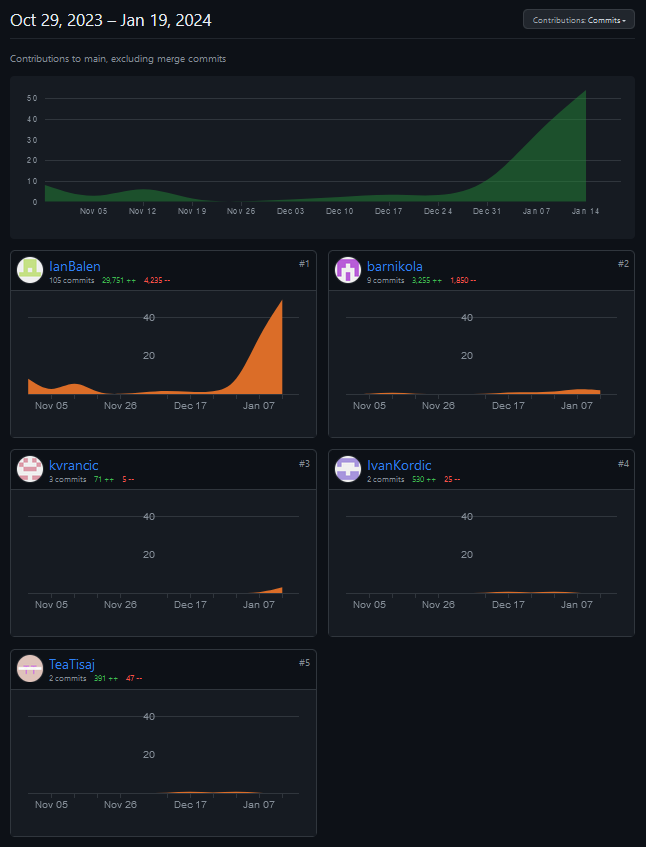
\includegraphics[width=\textwidth]{slike/backendGitHub.png} 
 		   \caption{Dijagram pregleda promjena \textit{backend} repozitorija}
 		   \label{fig:my_image}
		\end{figure}

		\begin{figure}[h!]
		    \centering
 		   \includegraphics[width=\textwidth]{slike/frontendGitHub.png} 
		    \caption{Dijagram pregleda promjena \textit{frontend} repozitorija}
 		   \label{fig:my_image}
		\end{figure}
		
	
		\begin{figure}[h!]
 		   \centering
  		  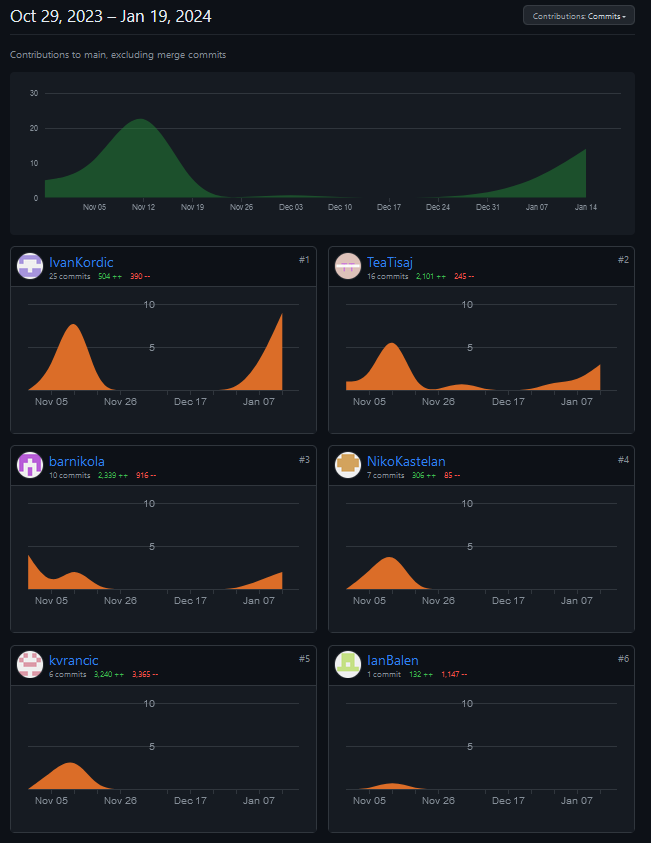
\includegraphics[width=\textwidth]{slike/documentationGitHub.png} 
   		 \caption{Dijagram pregleda promjena \textit{documentation} repozitorija}
   		 \label{fig:my_image}
		\end{figure}
		\eject
  
		
	
